\section{Introduction}


\begin{frame}[t]
    \frametitle{Introduction}
    % \begin{center}
    %     Elliptic curve are today's trend in cryptography. It is broadly use in signature
    %     authentification and secret key-sharing.
    % \end{center}

    % \begin{flushleft}
    %     Today's topic is about the group of rationales points of an elliptic curve and how to
    %     understand the underlying mechanism of its construction in order to give an example
    %     of a broadly use protocol in key sharing which is the Diffie-Hellman protocol. 
    % \end{flushleft}
    \begin{minipage}[t]{0.5\linewidth}
    \begin{itemize}
        \item What do we need to construct the group ?
        \item How to construct the group ?
        \item What are its application in cryptography ?
        \item Why does it work ? 
        \item What are the cons and pros ?
    \end{itemize}
    \end{minipage}%
    \hfill%
    \begin{minipage}[t]{0.3\linewidth}
        \begin{figure}[h]
            \centering
            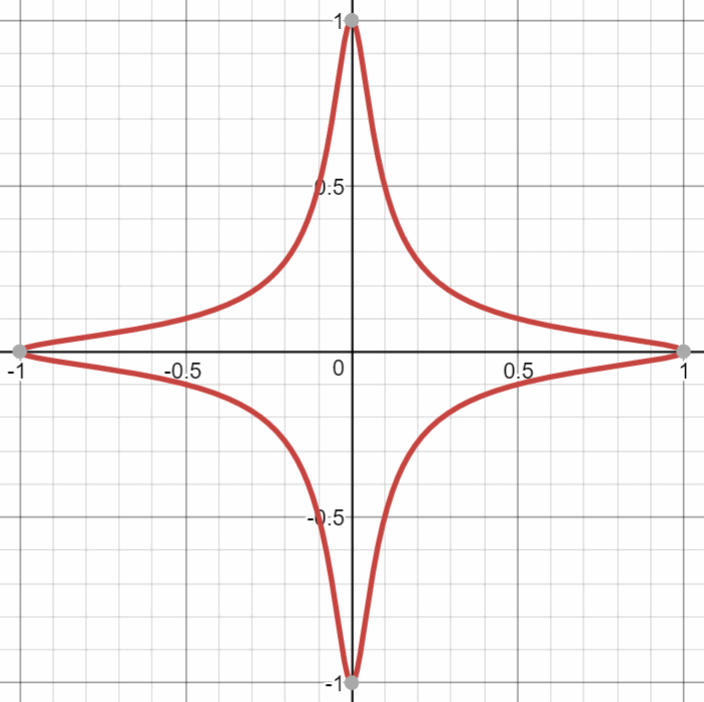
\includegraphics[width=0.8\textwidth]{edwardsCurve}
            \caption{Edwards' Curve : $x^2 + y^2 = 1 + 300x^2y^2$}
            \label{fig:edwardsCurve}
        \end{figure}
    \end{minipage}
\end{frame}
